
\section{Technische Umsetzung der Simulationsumgebung}
Zum Erlernen autonomer Fahrverhaltensweisen wird ein Simulator anhand der Beschreibung
aus Abschnitt \ref{sec:SimEnv} in Python umgesetzt. Das sehr ähnliche Projekt \emph{RobotSF}
der Universität Triest von Caruso et. al \cite{machines11020268} wird hierfür als Basis verwendet
und entsprechend adaptiert. In der ursprünglichen Version von \emph{RobotSF} steht sowohl
ein steuerbares Fahrzeug mit entsprechender Sensorik und Aktuatorik, als auch die
Simulation der Fußgänger mittels Social Force durch das Paket \emph{PySocialForce}
\cite{gao2020pysf} bereit. Die Implementierung des Simulators bezüglich der Differential
Drive Kinematik, des LiDAR-Sensors, der Fußgängersteuerung und der Kollisionslogik ist
von Caruso et. al und wird entsprechend der Konzeption aus Abschnitt \ref{sec:SimEnv} angepasst.
Die Schnittstelle der Simulationsumgebung zur Umsetzung der Trainingsalgorithmen von
Caruso et. al wird zugunsten einer breiteren Kompatibilität mit Implementierungen gängiger
Trainingsalgorithmen wie beispielsweise \emph{Stable Baselines 3} \cite{raffin2021sb3}
zu einer \emph{OpenAI Gym} Schnittstelle \cite{brockman2016openai} umgestellt. Da es sich
bei der Umsetzung der Simulationsumgebung um eine Erweiterung handelt, wird diese
im Folgenden \emph{RobotSF} genannt.

\subsection{Visualisierung der Simulationsumgebung}
Da die ursprüngliche Simulationsumgebung über keine Live-Visualisierung verfügt,
wird eine entsprechende Komponente zu \emph{RobotSF} hinzugefügt, wie in Abbildung
\ref{fig:SimPyGame} zu sehen ist. Die Ansicht verwendet die Visualisierungstechnologie
\emph{PyGame}, womit eine ausreichende Performanz für die flüssige Darstellung von
Bewegungen erzielt werden kann. Vergleichbare Technologien wie \emph{Tkinter} oder
\emph{Turtle} sind zu langsam und kommen daher nicht in Betracht.\\

\begin{figure}[h]
  \centering
  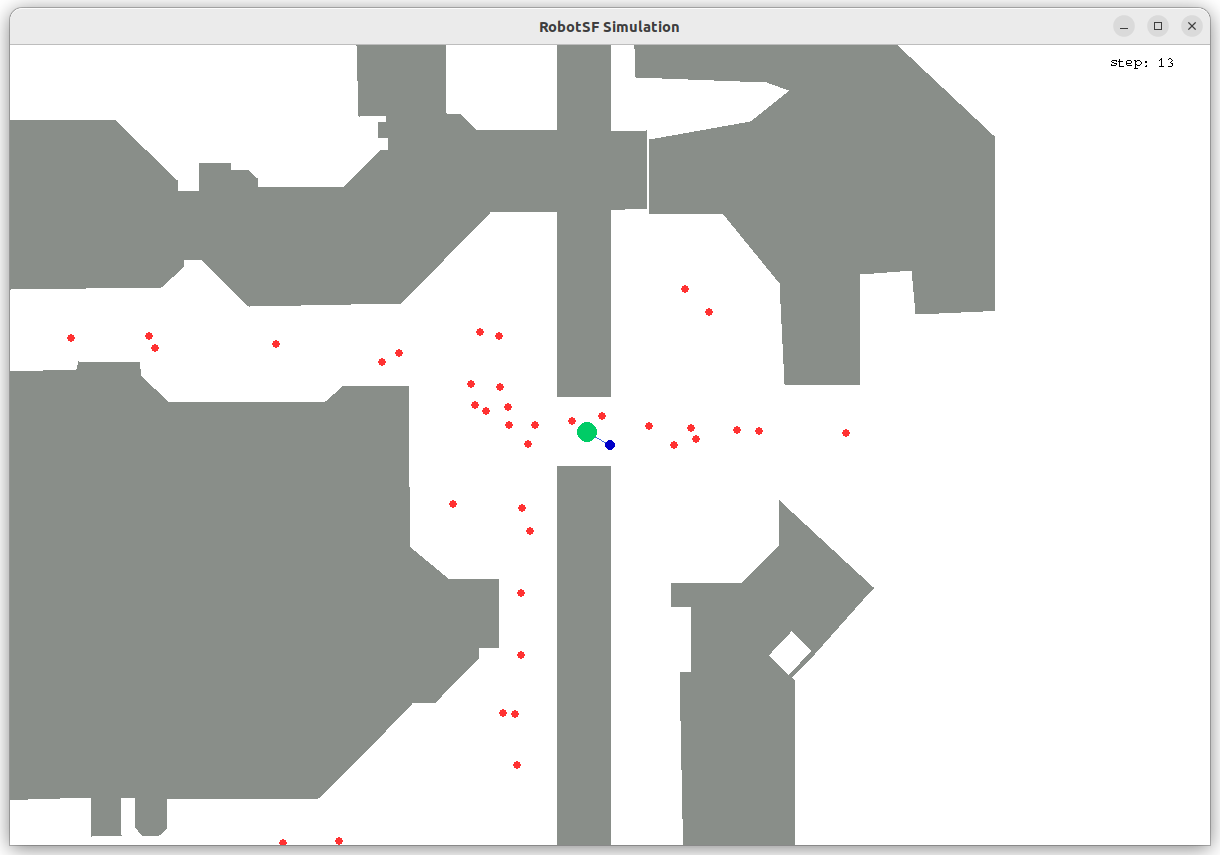
\includegraphics[width = 0.65\textwidth]{imgs/simulator_reworked}
  \caption{Simulatoranzeige mit PyGame}
  \label{fig:SimPyGame}
\end{figure}

Die dargestellten Entitäten umfassen das Fahrzeug (blauer Kreis), Fußgänger (rote Kreise)
und Hindernisse (graue Polygone). Zudem werden die Zielzonen der anzusteuernden
Wegpunkte (grüne Kreise) und der Dynamikvektor des Fahrzeugs (blaue Linie)
augmentiert. Die Kamera blickt senkrecht von oben auf die simulierte 2D-Ebene
und zentriert das betrachtete Fahrzeug in der Mitte des Bildschirms. Zudem kann
auch der Zoom-Faktor zu Beginn der Simulation passend eingestellt werden.\\

\subsection{Aufbereitung des Kartenmaterials}
Zur Bearbeitung des Kartenmaterials wird das Werkzeug \emph{Map Editor} entwickelt.
Wie in Abbildung \ref{fig:MapEditor} zu sehen ist, besteht der \emph{Map Editor} aus einem
Texteditor auf der linke Seite und einer Live-Vorschau der Karte auf der rechte Seite,
sodass mit vertretbarem Aufwand neue Trainingsszenarien erstellt werden können. Durch ein
weiteres Skript können Gebäudeumrisse maßstabsgetreu aus OpenStreetMap geladen werden,
was das Importieren von echtem Kartenmaterial auf einfache Weise ermöglicht. Per Linksklick
in die Vorschauanzeige werden die Koordinaten an der entsprechenden Stelle auf der Karte
ausgegeben, sodass sich Zonen und Routen leicht einpflegen lassen.\\

\begin{figure}[h]
  \centering
  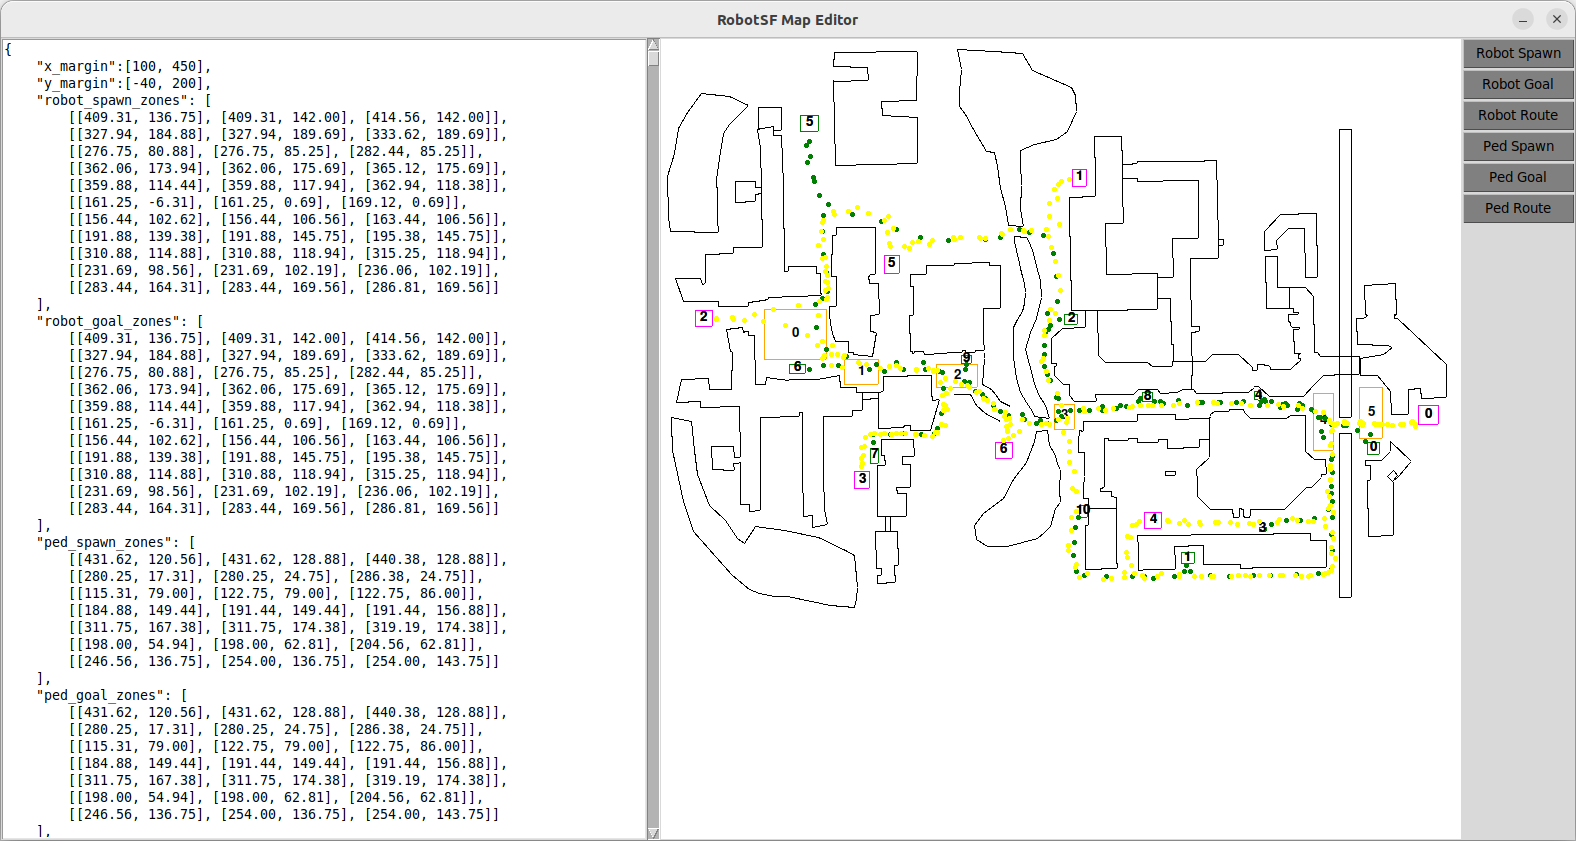
\includegraphics[width = 1.0\textwidth]{imgs/map_editor}
  \caption{Map Editor mit Texteingabe auf der linken und Vorschau auf der rechten Seite.
           Die Vorschau zeigt den Campus der Universität Augsburg. Im Text Editor
           wird das Kartenmaterial bearbeitet.}
  \label{fig:MapEditor}
\end{figure}

Für den Map Editor wird Tkinter als Visualisierungstechnologie gewählt,
da PyGame über keine vorgefertigten Bausteine zur Texteingabe verfügt und somit
ausscheidet. Zudem erfordert die Vorschau des Kartenmaterials ohnehin keine hohen
Bildraten für eine flüssige Darstellung, sodass stattdessen auf die Canvas-Funktion
von Tkinter zurückgegriffen wird. Ein vollkommen visuelles Bedienkonzept ohne
die Notwendigkeit einer manuellen Bearbeitung des Kartenmaterials im Texteditor stellt
eine Alternative dar, wird jedoch aufgrund des niedrigen Mehrwerts bei gleichzeitigem,
erheblichem Mehraufwand für das Projekt verworfen.
Es wäre vorgesehen gewesen, die einzelnen Zonen, Wegpunkte und Hindernisse per Mausklick
einzufügen. Per Schaltfläche wählt der Bearbeiter die einzufügende Struktur aus.
Anschließend setzt er die Umrisse per Linksklick in die Kartenvorschau. Ein Rechtsklick
bricht das Einfügen ab. Ist keine Schaltfläche aktiv, werden die Entitäten beim Bewegen
des Mauszeigers über ihre unmittelbare Umgebung hervorgehoben. Wird während der
Hervorhebung zusätzlich ein Recktsklick ausgeführt, löscht dies die Entität. Das Setzen
der Kartenumrisse löscht immer die vorherigen Umrisse. Per Drehung des Mausrads
kann wie gewöhnlich gezoomt werden.\\
